% !TEX root = Main.tex

\section{Vorgehen während der Entwicklung}
In diesem Kapitel wird näher auf die Entwicklung der geforderten Features des Compilers (vgl. \textit{\ref{sec:anforderungen} Anforderungen}) sowie dabei aufgetretene Probleme und deren Lösungen eingegangen.
%lass einfach das kapitel Probleme scrappen, da hier ja auch schon darauf eingangen wird

\subsection{Erste Schritte: Auswertung von arithmetischen Ausdrücken}
\label{subsec:arithExp}
% TO-DO: Kapitelnummer einfügen und prüfen
% kapitel 5 ist hier doch falsch????
Der Vorgehensweise unter \textit{\ref{sec:grundsatz}. Allgemeiner Grundsatz} entsprechend, implementierten wir zuerst die unserer Sicht nach grundlegendste Fähigkeit einer Programmiersprache: das Auswerten von arithmetischen Ausdrücken. Es soll möglich sein, Ausdrücke, die die Grundrechenarten sowie eine beliebig tiefe Schachtelung von Klammern enthalten, zu erkennen und der Operatorenpriorität entsprechend die gelesenen Tokens in einem Syntaxbaum zusammenzuführen. Dazu formulierten wir folgende Grammatik:


\scriptsize\begin{lstlisting} [frame=single] 
//Datei: Arithmetic.g4
grammar Arithmetic;

///////////////////////////////////////////////////////
// beliebige Folge der Ziffern 0 bis 9
INTEGER : [0-9]+ ;        
// ueberspringt Leerzeichen, Tabstops sowie Linefeeds
WS : [ \t\r\n]+ -> skip ; 
// oeffndende runde Klammer
LPAREN : '(';		  	  
// schliessende runde Klammer
RPAREN : ')';		  	  
///////////////////////////////////////////////////////
//mathematische Operatoren
PLUSOP : '+';
MINOP : '-';
MULTOP : '*';
DIVOP : '/';
///////////////////////////////////////////////////////
//Regeln fuer math. Ausdruecke
expression: INTEGER					
	| LPAREN expression RPAREN		
	| expression DIVOP  expression  
	| expression MULTOP expression	
	| expression MINOP  expression 
	| expression PLUSOP expression 
	;			
///////////////////////////////////////////////////////

\end{lstlisting}
\normalsize
Eine Grammatik für ANTLR hat folgenden Aufbau:

Die Definition der Grammatik beginnt mit dem Schlüsselwort ''grammar'' sowie dem Namen der Grammatik. Dabei gilt es zu beachten, dass die Datei den gleichen Namen wie die Grammatik selbst sowie die Dateiendung ''.g4'' besitzt. Diese Deklaration wird mit einem Semikolon abgeschlossen.

Zeilen, die mit ''//'' beginnen, sind Kommentare und haben keinen Einfluss auf die Grammatik. Sie dienen lediglich als Erläuterungen und zur Formatierung, um die Lesbarkeit zu verbessern.

Auf die Deklaration dürfen beliebig viele Regeln für die Grammatik folgen. Zur Formulierung der Regeln werden reguläre Ausdrücke genutzt. Beispielsweise besagt die sechste Zeile, dass es eine Regel INTEGER gibt, wobei ein INTEGER sich aus einer beliebigen Folge der Ziffern von 0 bis 9 zusammensetzt. Der reguläre Ausdruck [0-9] gibt an, dass ein beliebiges Zeichen im Bereich von 0 bis 9 vorkommen darf. Das abschließende ''+'' bedeutet, dass es sich um eine Kette dieser Zeichen, die beliebig lange ist, jedoch mindestens die Länge 1 besitzt, handelt.

Die Regel WS (Whitespace) besagt, dass bestimmte Zeichen, die nur der Formatierung dienen, ignoriert werden, da sie für das Übersetzen einer Quelldatei keine Bedeutung haben.

Die darauffolgenden Regeln sind Aliase für die Zeichen, die in arithmetischen Ausdrücken verwendet werden. Diese Auslagerung steigert unseres Erachtens nach die Lesbarkeit der letzten Regeln dieses Beispiels, sind aber nicht zwingend notwendig.

Die wohl relevanteste Regel trägt den Namen ''expression'' und legt fest, wie sich ein arithmetischer Ausdruck zusammensetzen kann. Im Vergleich zu den vorherigen Regeln, wurde hier von der Möglichkeit, mehrere alternative Möglichkeiten anzugeben, Gebrauch gemacht. Die Regel besagt, dass ein arithmetischer Ausdruck entweder aus 
\begin{itemize}
\item einer Zahl,
\item einem geklammerten Ausdruck,
\item einer Division mit zwei Operanden,
\item einer Multiplikation mit zwei Operanden,
\item einer Subtraktion mit zwei Operanden
\item oder einer Addition mit zwei Operanden
\end{itemize}
besteht.
Durch die Rekursion (die Regel verweist auf sich selbst) ist eine beliebige Länge des Ausdruckes möglich.

Eine Besonderheit, die zu beachten ist, besteht in der Rangfolge der Operatoren. Die höchste Bindung besitzt ein geklammerter Term, die nächst stärkere Bindung Divisionen und Multiplikationen. Die schwächste Bindung besitzen Subtraktionen und Additionen.

Damit diese Priorität gewährleistet werden kann, sind die Regeln in dieser bestimmten Reihenfolge notiert. ANTLR versucht immer zuerst die ''oberste'' Regel anzuwenden, daraufhin die darunter stehende usw.. Deshalb wird der folgende Ausdruck 

\begin{lstlisting} [frame=single]
2*10-48*(4-1)-16/4
\end{lstlisting}

zu diesem Syntaxbaum aufgelöst:

\begin{figure}[h!]
\centering
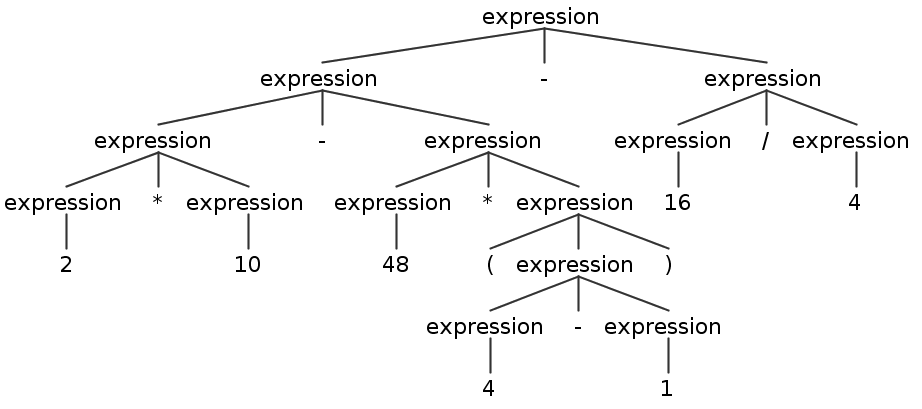
\includegraphics[scale=0.4]{pics/antlr4_parse_tree_arithmetic.png}
\caption{Syntaxbaum für beispielhaften arithmetischen Ausdruck}
\end{figure}

Des Weiteren ist zu beachten, dass arithmetischen Ausdrücke gleicher Operatorenpriorität von links  nach rechts ausgewertet werden müssen. Als Beispiel lässt sich hier der Term 
\begin{lstlisting} [frame=single]
8-5+2
\end{lstlisting}
nennen. Sowohl die Subtraktion als auch die Addition besitzen die gleiche Bindung. Wenn man hier fälschlicherweise zuerst die Addition, also 5+2, was 7 ergibt, auswertet und das Ergebnis dieser Operation von 8 subtrahiert, erhält man als Gesamtergebnis 1. 
In der korrekten Reihenfolge erfolgt zuerst die Subtraktion, also 8-5, was 3 ergibt, und erst darauf die Addition von 1, was als Gesamtergebnis 4 liefert. 
Um diese Fehlerquelle auszuschließen, sind in unserer Grammatik die Regel für Subtraktion vor der für Addition und die Regel für Division vor der für Multiplikation definiert. Da bei reinen Additionen bzw. reinen Multiplikationen die Auswertungsreihenfolge tatsächlich keine Rolle spielt, eine Subtraktion jedoch vor einer Additionen (vgl. Beispiel oben) ausgewertet werden muss, sorgt die Reihenfolge der Regeln in der Grammatik für eine korrekte Auswertung.

Ein analoges Beispiel zu Divisionen und Multiplikationen ist
\begin{lstlisting} [frame=single]
8/2*4
\end{lstlisting}
Auch hier ergibt sich ein ähnliches Problem wie beim vorherigen Beispiel. Wird zuerst die Multiplikation (2*4) ausgeführt und erst danach die Division (also 8/8 in diesem Fall), ist das Endergebnis 1 und nicht wie in der richtigen Reihenfolge 16.

Nach diesen Schritten sind wir also in der Lage einen Syntaxbaum zu erstellen. Der nötige Programmcode dafür wird von ANTLR automatisiert erstellt. Dabei ist die Eingabe dieses Programmes der auszuwertende Ausdruck. Die Ausgabe ist der Syntaxbaum, der zu Testzwecken auch als Grafik (vgl. Abbildung oben) ausgegeben werden kann. 

Der nächste wichtige Schritt der Übersetzung besteht nun in der Auswertung dieses Baumes. Dazu wird der Baum als Datenstruktur betrachtet. ANTLR liefert dabei mehrere Methoden, die auf Instanzen der Klasse ''ParseTree'' angewandt werden können. 
Jedes Token, das in der Grammatik definiert wurde und durch einen Knoten im Baum repräsentiert wird, besitzt eine sogenannte Visit-Methode. Diese Methode gibt eine Kette mit Zeichen zurück, wobei diese Zeichenkette die Anweisungen in der Zielsprache (Jasmin) enthält. Das Abarbeiten dieser Visit-Methoden in der richtigen Reihenfolge bildet die Grundlage für die Übersetzung, da hiernach alle Instruktionen in der Zielsprache zusammengesetzt sind. Was genau in einer Visit-Methode passiert, wird vom Entwickler festgelegt. ANTLR stellt sogehesen nur eine Vorlage zur Verfügung.

Um diese korrekte Reihenfolge zu gewährleisten, muss eine Anfangsregel (Startaxiom) festgelegt sein. In diesem Beispiel wurde festgelegt, dass der Programmstart - sprich der Wurzelknoten des Baumes - eine ''expression'' sein muss. Das bedeutet, das zunächst die Visit-Methode des Wurzelknoten aufgerufen wird. Damit nun auch die inneren Knoten des Syntaxbaums berücksichtigt werden, ist der Aufruf einer weiteren von ANTLR generierten Methode notwendig. Jeder Knoten des Baum besitzt eine visitChildren()-Methode, welche die entsprechenden Visit-Methoden der untergeordneten Knoten aufruft.

Um diese rekursive Vorgehensweise verständlicher zu machen, folgt ein Beispiel.


\begin{lstlisting} [frame=single]
/**@brief
 * verarbeitet Additionen
 */
public String visitAddition(AdditionContext ctx) {
	return visitChildren(ctx) + "\n"
		+ "iadd\n";
}
\end{lstlisting}
\pagebreak
Die Tatsache, dass es eine Methode visitAddition mit diesem Eingabeparameter und diesem Rückgabewert gibt, geht auf ANTLR zurück. Der Funktionsrumpf wurde jedoch von uns verfasst.

Zunächst werden die Kind-Knoten der Addition, sprich die Operanden, besucht. Wenn die Operanden aus weiteren mathematischen Operationen bestehen, werden zunächst diese aufgerufen, um die beliebige Länge von Ausdrücken zu ermöglichen. Handelt es sich bei einem Operanden um eine Zahl, wird die Methode visitNumber() aufgerufen.

\begin{lstlisting} [frame=single]
/**@brief
 * verarbeitet ganze Zahlen
 */
public String visitNumber(NumberContext ctx) {
	return "ldc " + ctx.getChild(0) + "\n";
}
\end{lstlisting}

Der Befehl \textit{ldc} steht für \textit{load constant} und ist die Jasmin-Instruktion, um einen Wert auf den Stack zu legen. \textit{ctx.getChild(0)} sorgt dafür, dass der Wert aus dem entsprechenden Knoten aus dem Baum entnommen wird.
Der Befehl \textit{iadd} in der visitAddition()-Methode steht für \textit{integer addition} und ist die Jasmin-Anweisung, zwei ganzzahlige Werte vom Stack zu nehmen, diese zu addieren und schließlich das Ergebnis wieder auf den Stack zu legen.

Der Compiler-interne Ablauf für die Übersetzung des Ausdruck 
\begin{lstlisting} [frame=single]
2 + 4
\end{lstlisting}
wäre also wie folgt: \\

Nach der lexikalischen und syntaktischen Analyse liegt folgender Syntaxbaum vor:

\begin{figure}[h!]
\centering
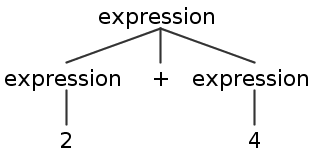
\includegraphics[scale=0.4]{pics/antlr4_parse_tree_visitAdditionVisitNumberBeispiel.png}
\caption{Syntaxbaum für beispielhaften arithmetischen Ausdruck}
\end{figure}
\pagebreak
Zunächst wird die visitAddition-Methode aufgerufen, da der Operator der expression das ''+'' Zeichen ist. Die visitChildren-Methode gibt nun die Zeichenkette
\begin{lstlisting} [frame=single]
ldc 2
ldc 4
\end{lstlisting}
zurück, da die untergeordneten Expressions nur Zahlen enthalten. Dem fügt die visitAddition-Methode wiederrum den Befehl
\begin{lstlisting} [frame=single]
iadd
\end{lstlisting}
hinzu, um die Addition durchzuführen.
\linebreak

In der JavaVM werden diese Instruktionen wie folgt verarbeitet:
Im Initialzustand ist der Stack leer.

\begin{figure}[h!]
\centering
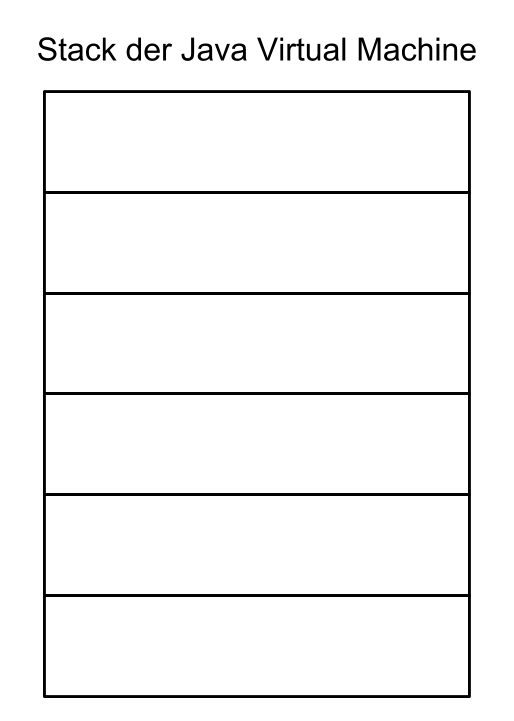
\includegraphics[scale=0.2]{pics/stack_visual.png}
\caption{Zustand des Kellerspeicher der JavaVM}
\end{figure}

Der Befehl \textit{ldc 2} legt den Wert \textit{2} auf den Stack.

\begin{figure}[h!]
\centering
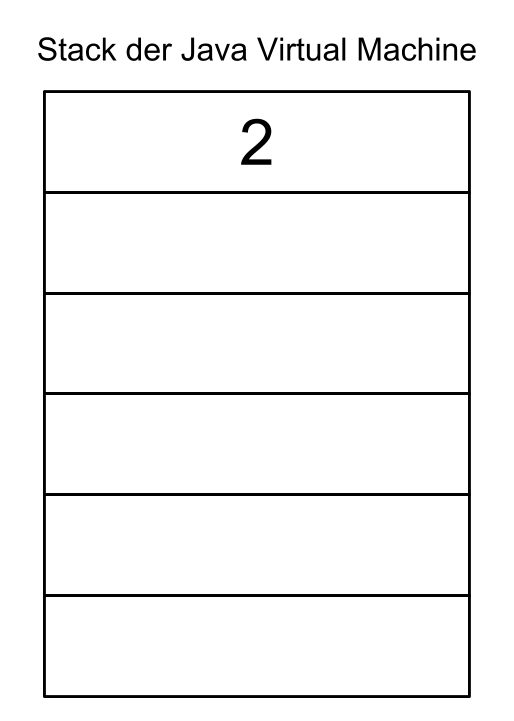
\includegraphics[scale=0.2]{pics/stack_visual(1).png}
\caption{Zustand des Kellerspeicher der JavaVM}
\end{figure}

Der Befehl \textit{ldc 4} legt den Wert \textit{4} auf den Stack.

\begin{figure}[h!]
\centering
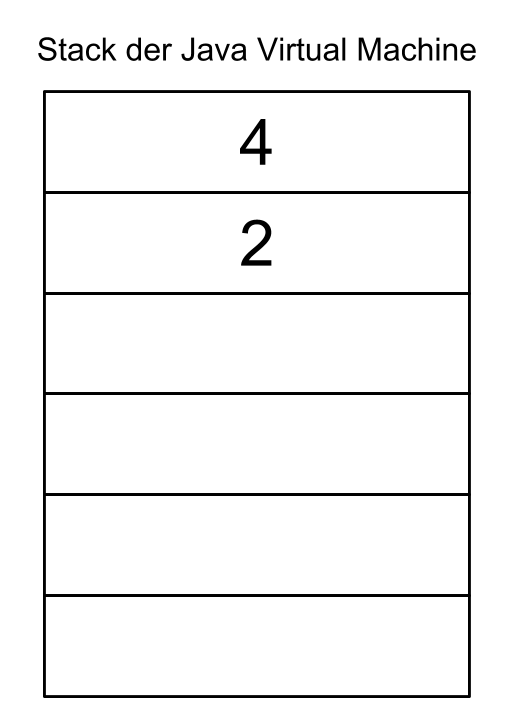
\includegraphics[scale=0.2]{pics/stack_visual(2).png}
\caption{Zustand des Kellerspeicher der JavaVM}
\end{figure}

Der Befehl \textit{iadd} nimmt zwei Werte vom Stack und legt das Ergebnis der Addition dieser Werte wieder auf den Stack

\begin{figure}[h!]
\centering
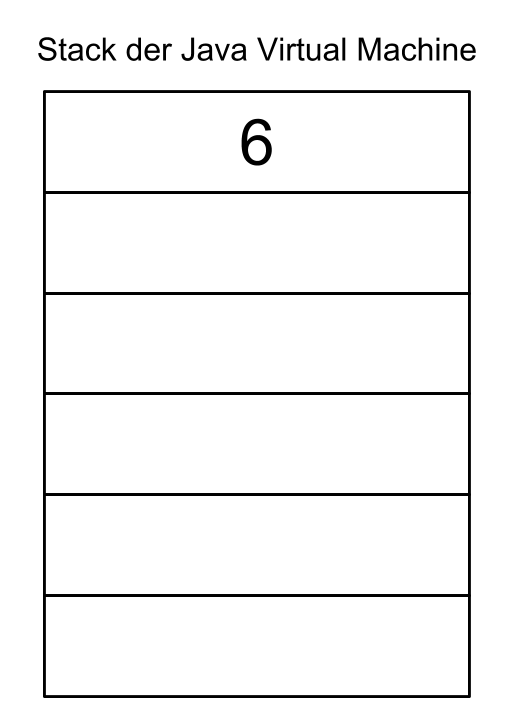
\includegraphics[scale=0.2]{pics/stack_visual(3).png}
\caption{Zustand des Kellerspeicher der JavaVM}
\label{fig:method}
\end{figure}



\pagebreak

\subsection{Ausweiten der simplen Grammatik}
Nachdem die Sprache grundlegende Funktionalität erhielt, versuchten wir die weiteren Bestandteile, die durch die Anforderungen festgelegt wurden, zu implementieren. 


\subsubsection{Ergebnisausgabe}
Ein Programm ohne Ausgabe ergibt keinen Sinn, da nie das berechnete Ergebnis betrachtet werden kann. Eine Ausgabefunktion zu implementieren stellte sich nicht als all zu großes Problem heraus, da Jasmin die Fähigkeit besitzt Objekte und Methoden in der Java Library zu nutzen. Wir implementierten dies Ausgabefunktion wie folgt:

\scriptsize \begin{lstlisting}[frame=single]
/**@brief
 * vearbeitet den Aufruf der println-Funktion
 */
public String visitPrintln(PrintlnContext ctx) {
	return  ";calling println\n" + 
		//legt ein System.out Objekt auf den Stack
		"getstatic java/lang/System/out Ljava/io/PrintStream;\n" + 	
		//Argument der print-Funktion
		visit(ctx.argument) + 						
		//ruft die Methode println des System.out-Objekts auf
		"invokevirtual java/io/PrintStream/println(I)V\n\n"; 				
}
\end{lstlisting}

\normalsize
Es wird zuerst ein System.out-Objekt auf den Stack gelegt, danach der auszugebende Wert. Schließlich folgt der Aufruf der Methode println(), die das Argument sowie das System.out-Objekt vom Stack wieder herunternimmt.


Der Aufruf in unserer Programmiersprache lautet: 
\begin{lstlisting}[frame=single]
println( argument );
\end{lstlisting}

\subsection{Implementierung von Variablen}
Eine Variable wird folgendermaßen deklariert:
\begin{lstlisting}[frame=single]
int name;
\end{lstlisting}
Wenn ein entsprechender Knoten im Syntaxbaum besucht wird, wird geprüft, ob bereits eine Variable mit dem selben Namen im aktuellen Gültigkeitsbereich existiert. Ist dies der Fall, wird eine Exception ausgelöst und der Kompiliervorgang mit einer entsprechenden Fehlermeldung beendet. Existiert der Name der Variablen im aktuellen Gültigkeitsbereich noch nicht wird ein neuer Eintrag in der Variablentabelle erstellt.

Um einer deklarierten Variable einen Wert zuzuweisen, wird folgende Syntax verwendet:
\begin{lstlisting}[frame=single]
name = EXPRESSION;
\end{lstlisting}
Dabei muss eine EXPRESSION zu einem Wert evaluierbar sein.
Wird ein Knoten mit einer Zuweisung besucht, erfolgt zuerst der Versuch den Namen der Variablen zu einem Index in der Variablentabelle aufzulösen. Gelingt dies nicht, bedeutet das, dass die Variable nicht deklariert wurde. Es wird eine enstprechende Exception ausgelöst. Kann der Name der Variablen zu einem Index aufgelöst werden, wird der Wert der Variable mit 
\begin{lstlisting}[frame=single]
istore [index]
\end{lstlisting}
vom Stack genommen und in der Jasmin-Variablentabelle gespeichert.

Wird auf eine Variable lesend zugegriffen, d.h. sie kommt im rechten Teil einer Zuweisung vor, so muss auch wieder der Name zu einem Index aufgelöst werden. Hierzu wird intern die gleiche Methode verwendet. Nach erfolgreichem Ermitteln des Index kann der Wert der Variable mit dem Befehl 
\begin{lstlisting}[frame=single]
iload [index]
\end{lstlisting}
wieder auf den Stack gelegt und somit verwendet werden.

\subsection{Implementierung von Funktionen}
Vor dem eigentlichen Aufruf des Visitors, wird der gesamte Baum auf Funktionsdeklarationen untersucht. Dies sorgt dafür, dass Funktionen an beliebigen Stellen im Quellcode definiert werden können und keine Vorwärtsdeklarationen notwendig sind. Die gefundenen Funktionen werden in einer Liste gespeichert.

%Funktionen werden mit folgender Syntax deklariert:
% ToDo: Bitte einfügen; 
%	siehe Kapitel Verwendung

Wird ein Knoten mit einer Funktionsdeklaration besucht wird zunächst in dieser Liste überprüft, ob eine Funktion mit der gleichen Signatur bereits existiert. Ist dies der Fall, wird eine Exception ausgelöst und der Kompiliervorgang abgebrochen. Andernfalls wird ein neuer Eintrag mit dem Namen und der Signatur der Funktion in die Funktionsliste eingefügt.
Die Signatur besteht dabei aus dem Namen und den übergebenen Parametern. Beispielsweise dürfen sowohl die Funktion
\begin{lstlisting}[frame=single]
int doSomething();
\end{lstlisting}
als auch die Funktionen
\begin{lstlisting}[frame=single]
int doSomething(int paramA);
int doSomething(int paramA, int paramB);
\end{lstlisting}
in der gleichen Quelldatei vorkommen, da sie sich in den Übergabeparametern unterscheiden.

Beim Aufruf von Funktionen wird ebenfalls geprüft, ob eine Funktion mit der gegebenen Signatur existiert. Existiert die Funktion nicht, wird eine Exception ausgelöst, andernfalls der Funktionsaufruf wie folgt verarbeitet. 
In einem String wird die Anweisungen für den Aufruf für Jasmin zusammengesetzt, wobei zunächst gegebenenfalls Variablen für die Übergabeparameter angelegt werden. 
Anschließend wird der Aufruf in Jasmin-Syntax generiert.

\begin{lstlisting}[frame=single]
invokestatic [objektname]/[funktionsname]([parameter])[rueckgabetyp]
\end{lstlisting}

Der Objektname ist nur intern, also für die JVM relevant, da diese der Java-Philosophie entsprechend stark objektorientiert ausgerichtet ist. Es muss also nur darauf geachtet werden, dass der Objektname gleich dem der Jasmin-Main-Funktion ist.
Die Parameterliste besteht aus je einem ''I'' (für Integer) pro übergebenem Parameter.
Der Rückgabetyp wird wiederrum durch ein ''I'' für den Datentyp Integer angegeben. Da der einzige unterstützte Datentyp unserer Sprache ''int'' ist, ist der Rückgabetyp hardcodiert und damit für jede Funktion gleich.

Desweiteren wird bei einem Funktionsaufruf die aktuelle Variablentabelle kopiert und eine neue Variablentabelle für die Funktion angelegt. Dies ermöglicht verschiedene Gültigkeitsbereiche (engl. scopes). 
Beim Verlassen der Funktion wird die vorherige Variablentabelle wieder hergestellt.

\subsection{Implementierung von Konstanten}
Konstanten sind intern als Erweiterung von Variablen anzusehen. 
Zusätzlich zu Variablen werden bei Konstanten folgende Schritte ausgeführt:
Wird eine Konstante deklariert, wird deren hasBeenAssigned-Flag auf false gesetzt.
Bei der Wertzuweisung zu der Konstanten wird geprüft, welchen Wert dieses Flag besitzt. Ist der Wert false, wird eine normale Zuweisung durchgeführt und der Wert des Flags auf true gesetzt. Ist der Wert true, wurde der Konstanten bereits eine Wert zugewiesen, weshalb eine weitere Zuweisung nicht erfolgen darf. Es wird eine Exception ausgelöst und der Kompiliervorgang mit einer entsprechenden Fehlermeldung abgebrochen.

\subsection{Implementierung von Bedingten Verzweigungen}
Verzweigungen sind in drei Teile untergliedert:
\begin{itemize}
	\item conditionInstructions
	\item onTrueInstructions
	\item onFalseInstructions	
\end{itemize}

Die conditionInstructions enthalten die Auswertung eines mathematischen Ausdrucks, dessen Ergebnis einen Wahrheitswert repräsentiert. Der Wert 0 repräsentiert \textit{false}, alle anderen Werte werden als \textit{true} interpretiert.
 
Wird die Bedingung zu true evaluiert, werden die onTrueInstructions ausgeführt, die onFalseInstructions werden übersprungen. Andernfalls, werden die onTrueInstructions übersprungen und die onFalseInstructions ausgeführt.
Um die entsprechenden Instruktionen zu überspringen, werden Labels benötigt, die einen Sprung zu einer definierten Stelle im Proramm ermöglichen. Damit die Labels für jede Verzweigung eindeutig sind, wird gezählt, wie oft Verzweigungen vorkommen und die Labels entsprechend benannt.

\subsection{Implementierung einer Schleife}
Eine Schleife wird intern  in
\begin{itemize}
\item Bedingung
\item Befehle, die bei einer wahren Bedingung ausgeführt werden
\end{itemize}

Der folgende Pseudocode ist ähnlich zu entsprechenden Jasmin-Anweisungen :
\\
\begin{algorithm}[H]
	conditionLabel \\
	conditionInstructions \\
		\If{conditionInstructions == true}
		{ 
			Sprung zu onTrueLabel
		}
		\If{conditionInstruction == false}
		{
			Sprung zu endOfWhileLabel
		}
	[onTrueLabel] \\
	onTrueInstructions \\
	Sprung zu conditionLabel \\	
	endOfWhileLabel
\end{algorithm}
\(\)\\
Die Labels werden benötigt, damit in der Schleife an die entsprechende Stelle gesprungen werden kann. Damit intern die Labels zur richtigen Schleife zugeordnet werden können, wird mitgezählt, wie oft Schleifen im Programm verwendet werden.

\subsection{Dokumentation}
Zur effizienten Erstellung der Dokumentation wurde \LaTeX \(\) in Verbindung mit TexMaker verwendet. Dazu wurden die einzelnen Hauptüberschriften in eigene Dateien ausgelagert und in der Hauptdatei inkludiert. Dies hat eine erhöhte Übersichtlichkeit zur Folge.
Um die Dokumentation versioniert zu speichern, wurde diese im verwendeten Git-Repository hochgeladen. Damit keine unnötigen Entwicklungs- bzw. Zwischenschrittdateien von \LaTeX \(\) in das verwendete Git-Repository übernommen werden, wurde ein Alias erstellt, der ebendiese Dateien beim Alias-Aufruf automatisiert entfernt. Dieser Alias sieht wie folgt aus:

\begin{lstlisting}[frame=single]
rmtex_dev()
{
	echo "Removing .aux"
	rm *.aux &> /dev/null
	echo "Removing .toc"
	rm *.toc &> /dev/null
	echo "Removing .synctex.gz"
	rm *.synctex.gz &> /dev/null
	echo "Removing .log"
	em *.log &> /dev/null
	echo "Removing .out"
	rm *.out &> /dev/null
}
\end{lstlisting}

\subsection{Probleme im Projekt und Team}
Neben den bereits in anderen Kapiteln genannten Problemen mit Werkzeugen wie \textit{Eclipse}, bestand auch eine große Barriere im Team in der Zeiteinteilung. So ergaben sich zum Beispiel unterschiedliche Arbeitszeiten und Zeitspannen, in denen am Projekt gearbeitet werden konnte, was Absprachen und Besprechungen in die Länge zieht und nach unserer Erfahrung sehr mühsam macht.
